\chapter{Summary}
\label{ch:summary}
The presented thesis revolved around managing multiple Docker containers, each responsible for a part of the data pipeline, gathering and transforming card market information from a public website into a user-oriented analysis. The constraints and requirements described in sections \ref{s:functional_req} and \ref{s:nonfunctional_req} shaped the system to perform a series of robust tasks, in order to aid the potential buyer with novel market insights. In retrospect, the program does fulfill the following functional requirements:

\begin{enumerate}
    \item Gathering cards, sellers and offers' data and keeping it up to date --- realized by the \textit{data\_gathering} container, mostly with the use of scheduling flags and Selenium framework,
    \item Possibility to change the expansion --- it is a configurable variable in \textit{config.py} file of the gathering container,
    \item Saving the gathered entities into CSV files --- staging area,
    \item Continuous execution of every container,
    \item Once-per-day data update,
    \item Once-per-hour database update checks,
    \item Once-per-hour data mining run,
    \item Having a robust web application with four data analyses.
\end{enumerate}

Non-functional requirements were concerned with \textit{how} does the system behave, rather that \textit{what} it does. All of them have been fulfilled:
\begin{enumerate}
    \item Full data processing time is about 1.5-2.5 hours, given that all the sellers are saved. This requirement fails for the first run of the code, especially if the Internet connection and hardware setup are suboptimal.
    \item The system is standalone within the containerization software, the only prerequisite to running it is having Docker installed on the system. Has been tested on Fedora 35 with minimal setup to a triumphant success.
    \item The requests slow down after no proper response is detected, which is not dynamically chaning the requests timing, but rather giving the server a break to avoid running into error 429 Too Many Requests.
    \item No user input is required after running the system in order to keep it healthy, functional and up to date. The only interaction the user has is receiving the results and putting their conditions to find out what the best deal is.
\end{enumerate}

Overall, six containers were used, four of which were sub-projects acting on the data (data gathering, database managing, data mining, website serving). Additionally, a Sematext monitoring software was used to observe the performance of the system, which amounted to additional \textit{sematext\_agent} container, reporting execution details to the dashboard.

\section{Containers performance}
Using the free version of Sematext monitoring agent, the author was able to track the performance of the system, mainly the MySQL database. \par
In Fig. \ref{fig:mysql_network} we can see the amount of data received and transmitted by the database. The steady hourly level represents the data mining module, which connects to the database every 60 minutes to perform the analysis. Spikes around 1:00 am correspond to the database manager updating the tables with new data gathered from this day. \par
Fig. \ref{fig:mysql_performance} shows the load of the database. We can see the correlation between the Selects Rate and CPU and Memory load. Around 4 GB of memory are used, with additional 2--3 GB chached and buffered. \par
The last figure juxtaposes the number of tables dropped with tables created (Fig. \ref{fig:mysql_create_drop}). Due to the architecture of the system, each table is replaced by its new version, meaning every \texttt{CREATE} is paired with a \texttt{DROP}, which is reflected in the presented chart.

\begin{figure}
    \centering
    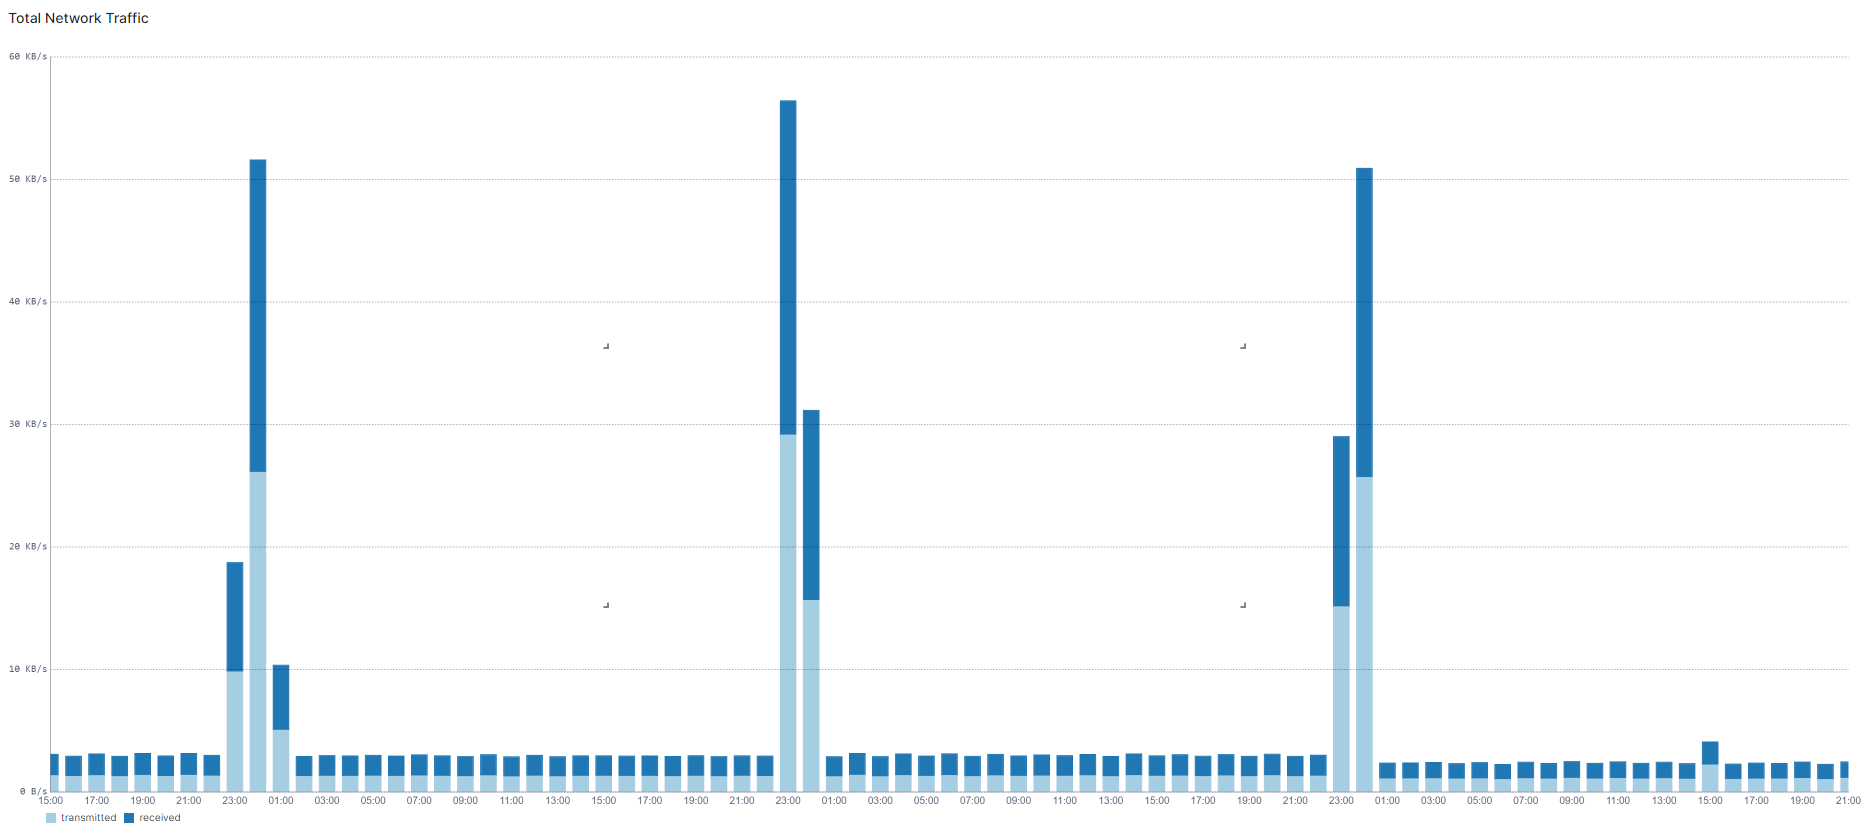
\includegraphics[width=\textwidth]{figures/mysql_network.png}
    \caption{}
    \label{fig:mysql_network}
\end{figure}

\begin{figure}
    \centering
    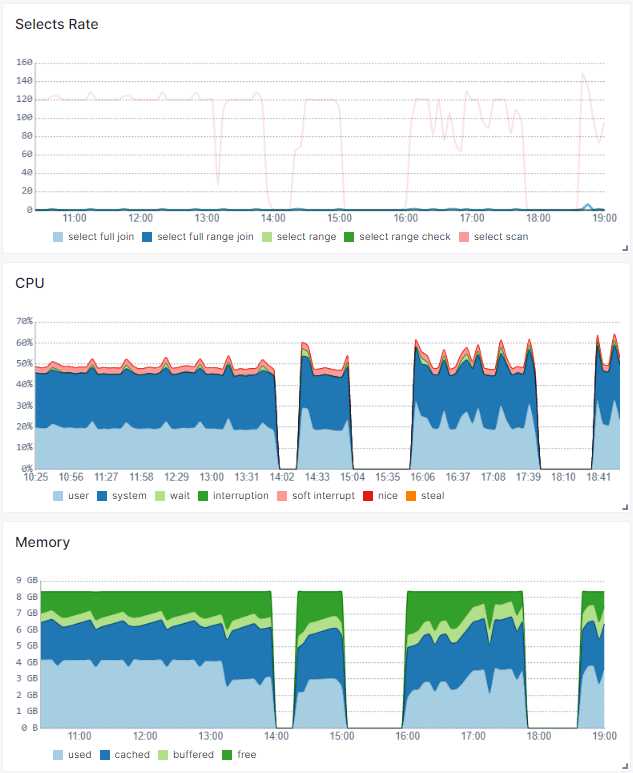
\includegraphics[width=\textwidth]{figures/mysql_performance.png}
    \caption{}
    \label{fig:mysql_performance}
\end{figure}

\begin{figure}
    \centering
    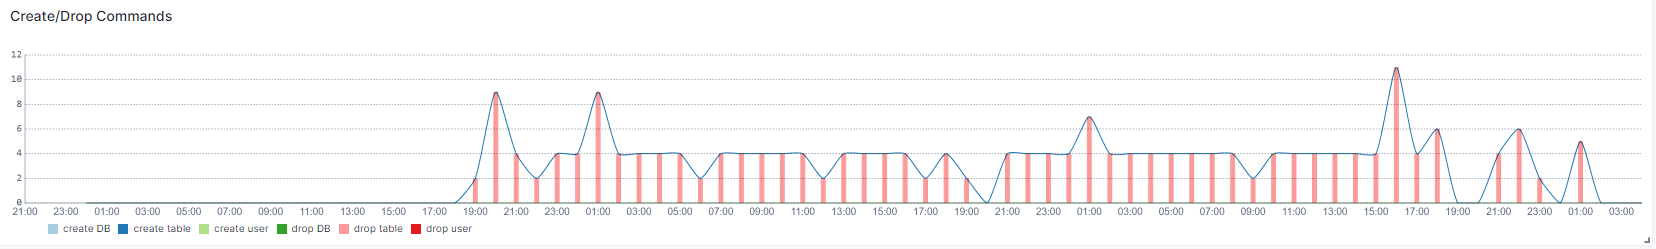
\includegraphics[width=\textwidth]{figures/mysql_create_drop.png}
    \caption{}
    \label{fig:mysql_create_drop}
\end{figure}


\section{Scaling and customizability}
The system was build with the idea of scalability from the very beginning. The number of gathered data can be extended to years, as long as the largest table can be loaded into a single dataframe without running out of memory. Interestingly, if the data gathering part was swapped with other code for data acquisition, the data warehouse could instead be focused around the new theme and still work with few minor changes to the other containers. One may want to choose another website, and if the information provided there is sufficient to create the same entities in CSV files, there would be no changes needed for the rest of the data pipeline to work correctly. Moreover, the usage of containers (which can be asynchonously stopped and started) suggests a version of the system with multiple versions of each container, each still doing their core task, but with differences. Such modular approach is seen more and more in the world of mordern technology and would be perfectly applicable here. Additionally, the acquired data can be used in a myriad of different ways besides those presented in this paper. The created data warehouse is simple, but proves to be a powerful tool, which usefulness can be extended far with the right approach and broad imagination.

\section{Conclusions}
In conclusion, the created project is a successfully working solution. It performes the totality of given tasks, works relatively fast, uses verbose logging and it set up to be resilient and easy to use. The data warehouse model fits well with the purpose of the program and containers allow to isolate the steps on the data pipeline, as well as transport the solution to any system and run it there. The results are calculated fast and often, and the web application provides answers to questions, which can substantially contribute to the user making a better market choice. Using the available technology the author was able to transform large, disseminated pieces of information into centralized and uniform data, to then extract insights in a matter of seconds, whereas the market research would have taken days, if not weeks, spent on browing the service websites. This sufficiently proves the real usefulness of today's technology and the advantage in hands of those who use it well. However, if data is the sword of the 21st century, one must always be cautious not to get cut; issues with big data are challanges many of the biggest companies face today, and the ethics of discovering knowledge about people, which even they do not have, opens a whole new Pandora's box of moral dilemmas. Just like the technology promising improvement in our lifestyles, data is a double-edged sword. It's giving us an advantage, but is also placing a great burden of responsibility --- a burden, which has to be carried to the end once the lid is opened.
